\documentclass{article}
\usepackage{graphicx}
\usepackage{caption}
\begin{document}

\title{Playlist Report}
\author{Name : Arsh Srivastava\\Roll number: AI22BTECH11003}
\date{\today}

\maketitle

\section{Introduction}
This report provides an overview and analysis of the playlist code implemented using the pygame library. The code allows users to play a randomized playlist of songs and provides options to control the playback, including skipping songs and stopping the playlist.

\section{Code Explanation}

The code is structured into several functions and a main loop. Here's a breakdown of the code's key components:

\subsection{Importing Libraries}
The code begins by importing the necessary libraries, including pygame and numpy. These libraries are used for audio playback and generating random numbers, respectively.

\subsection{Song Playback}
The \texttt{play\_song} function is responsible for loading and playing a given song file. It utilizes the pygame.mixer.music module to load the song and initiate playback.

\subsection{Playlist Generation and Playback}
The \texttt{my\_playlist} function manages the generation and playback of the playlist. It initializes the pygame mixer and creates an empty list, \texttt{my\_list}, to keep track of played songs. The function uses an infinite loop to continuously play songs.

Inside the loop, a random number between 1 and 20 is generated using numpy's \texttt{randint} function. If the number is not in \texttt{my\_list}, it is added to the list, and the corresponding song is played using the \texttt{play\_song} function.

While the song is playing, the code prompts the user with a question asking if they want to skip the current song. If the user responds with "yes," the song is stopped, and the loop proceeds to the next iteration.

After the song finishes playing, the code asks the user if they want to stop the playlist. If the user responds with "yes," the playback is stopped, and the pygame mixer is closed.

\subsection{Main Loop}
The code includes a main loop that calls the \texttt{my\_playlist} function five times, allowing for the generation and playback of multiple playlists.

\section{Conclusion}
The implemented code provides a simple and interactive way to play randomized playlists and control the playback of songs. It leverages pygame's audio capabilities and numpy's random number generation to create a dynamic playlist experience for the user.

\begin{figure}[h]
\centering
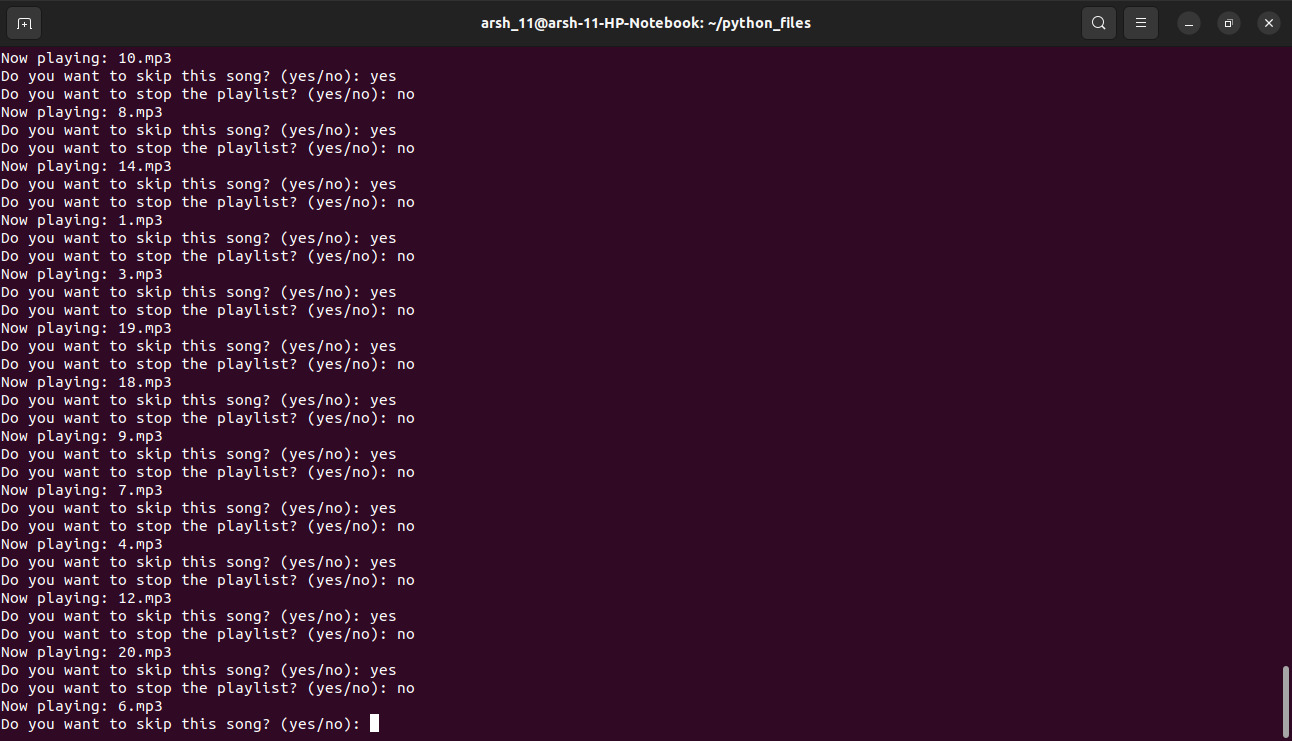
\includegraphics[width=0.5\textwidth]{figures/pic1.jpeg}
\caption{Image of 20 pics}
\label{fig:my_label}
\end{figure}
\begin{figure}
\centering
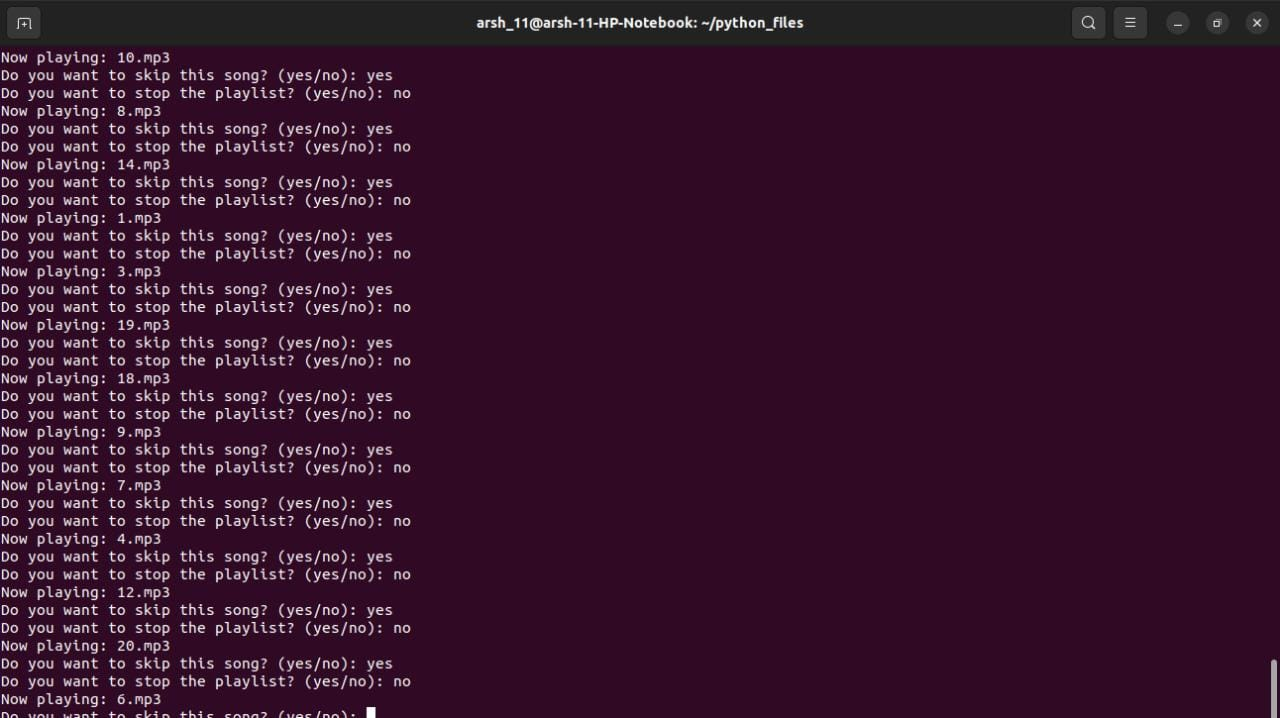
\includegraphics[width=0.5\textwidth]{figures/pic2.jpeg}
\caption{Image of 20 pics continued}
\label{fig:my_label}
\end{figure}

\end{document}